\documentclass[letterpaper,landscape]{slides}
%\documentclass[letterpaper,portrait]{slides}
\usepackage{boxedminipage}

%\input /u/rhl/TeX/pdf.tex
\input pdf.tex

\newif\ifTalk\Talktrue		% We generating a talk, not printing
%\Talkfalse			% no; we're really printing

%\pagestyle{empty}
\setlength{\topmargin}{-1in}
\setlength{\textheight}{7.5in}
\setlength{\textwidth}{9in}
\setlength{\oddsidemargin}{0pt}
\setlength{\oddsidemargin}{0pt}

%\onlyslides{1-3,4,10-9999}
%\onlyslides{26-9999}

\begin{document}

\newcommand{\XXX}[1]{\textbf{XXX} #1}
\newcommand{\colour}[1]{\color{#1}}

\def\eq#1{\begin{equation} \color{blue} #1 \end{equation}}

\def\b#1{{\bf  #1}}
\def\p{\partial}
\def\th{^{th}}
\def\msun{{\rm\,M_\odot}}
\def\bnabla{{\bf\nabla}}
\def\dint{\int\!\!\!\int}
\def\d{{\rm d}}
\def\i{{\rm i}}
\def\ddt#1{{\rm{d} #1\over {\rm dt}}}
\def\ddtS#1{{\rm{d^2} #1\over {\rm dt^2}}}
%\lta and \gta produce > and < signs with twiddle underneath
\def\spose#1{\hbox to 0pt{#1\hss}}
\def\lta{\mathrel{\spose{\lower 3pt\hbox{$\mathchar"218$}}
     \raise 2.0pt\hbox{$\mathchar"13C$}}}
\def\gta{\mathrel{\spose{\lower 3pt\hbox{$\mathchar"218$}}
     \raise 2.0pt\hbox{$\mathchar"13E$}}}
\def\mspace{\hbox{\quad}}

\def\deffn#1{{\bf#1}}\def\eqs#1{equations \rf#1}


\newcount\itemCnt\itemCnt=0
\newcommand{\nitem}{%
  \global\advance\itemCnt by 1
  ~\vskip0cm\the\itemCnt.\qquad}

\definecolor{orange}{rgb}{1.0, 0.5, 0.0}
\definecolor{purple}{cmyk}{0.4, 0.8, 0.3, 0.0}

%%%%%%%%%%%%%%%%%%%%%%%%%%%%%%%%%%%
\newcommand{\picslide}[7]{%
  \begin{slide}
     \begin{center}
        \begin{minipage}{#5in}
            \hskip #6in
            \hskip -1in
            {\scalebox{#4}{\includegraphics{#1.#2}}}
            \vskip #7in~
            {\large \color{blue} #3}
        \end{minipage}
     \end{center}
     \vfill
  \end{slide}
}
%%%%%%%%%%%%%%%%%%%%%%%%%%%%%%%%%%%

%%%%%%%%%%%%%%%%%%%%%%%%%%%%%%%%%%%
\newcommand{\QAslide}[1]{%
  \begin{slide}
     \begin{center}
        \begin{minipage}{7in}
            \phantom{x} \vskip -0.7in
            \phantom{x} \hskip  0.5in
            {\scalebox{0.8} {\includegraphics{#1.pdf}}}           
        \end{minipage}
     \end{center}
 \end{slide}
}
%%%%%%%%%%%%%%%%%%%%%%%%%%%%%%%%%%%

%%%%%%%%%%%%%%%%%%%%%%%%%%%%%%%%%%%
\newcommand{\Spicslide}[7]{%
  \begin{slide}
     \begin{center}
        \begin{minipage}{#5in}
            \vskip #6in
            \hskip #7in
            {\scalebox{#4}{\includegraphics{#1.#2}}}
        \end{minipage}
     \end{center}
     \vfill
  \end{slide}
}
%%%%%%%%%%%%%%%%%%%%%%%%%%%%%%%%%%%
 
%%%%%%%%%%%%%%%%%%%%%%%%%%%%%%%%%%%
\newcommand{\onepic}[6]{%
\begin{slide}
     \begin{center}
        \begin{minipage}{#1in}
            {\large \color{blue} #6}
            \phantom{x} \vskip #2in
            \phantom{x} \hskip #3in
            {\scalebox{#4}{\includegraphics{#5}}}   
        \end{minipage}
     \end{center}
    \vfill
\end{slide}
}

\newcommand{\smgraphicsZI}[7]{
   \begin{minipage}[t]{#6in}
     \vskip#3in \hskip#4in
     \scalebox{#5}{\includegraphics{#1.#2}}
   \end{minipage}}


\newcommand{\palV}[2]{
\begin{slide}

\begin{minipage}{8in}
~\vskip-1in
\rotatebox{0}{\scalebox{0.85}{\includegraphics{#1}}}
\vskip -2.5in~
\end{minipage}

#2

\vfill
\end{slide}
}


%------------------------------------------------------------------------------
%------------------------------------------------------------------------------

\begin{slide}

\phantom{x}
\vskip -2in
\begin{center}
\bfseries
{\large {\color{blue} Astr 511: Galaxies as galaxies}}
\end{center}

{\centerline {{\color{blue} 
Winter Quarter 2017, University of Washington}}}
{\centerline {{\color{blue} 
Mario Juri\'{c} \& \v{Z}eljko Ivezi\'{c} }}}

\vskip 1.6in

{\centerline {\huge {\color{red}      Lecture 3:             }}}
\vskip 0.2in 
{\centerline {\Large {\color{blue} Basic properties of galaxies }}}

\vfill
\end{slide}
%------------------------------------------------------------------------------

%------------------------------------------------------------------------------

\begin{slide}
\begin{center}
{\large \color{red} 
                         Outline
}
\end{center}

\begin{itemize}
\item {\color{blue} A Little Bit of History}
\item {\color{blue} Galaxy Types and Classification}
\item {\color{blue} Galaxy Properties}
\begin{itemize}
\item Intensity profiles
\item Rotation curves 
\item Spiral arms 
\end{itemize}          
\end{itemize}          

\vfill
\end{slide}


%------------------------------------------------------------------------------



%------------------------------------------------------------------------------
% TWO-SIDED PAGE 
\begin{slide}

\hbox to \hsize{
\begin{minipage}[t]{9cm}
\begin{center}
\vskip -0.85in
\scalebox{0.72}{\hskip -1.5in 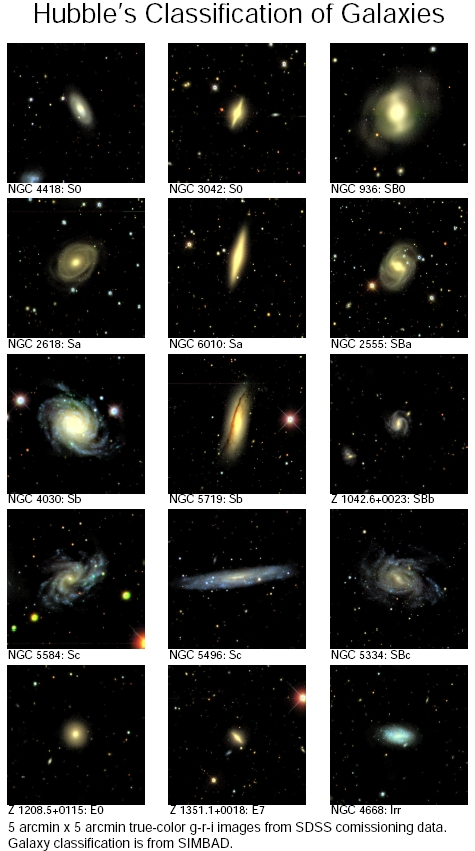
\includegraphics{figures/HubbleSDSS.jpg}}
\end{center}
\end{minipage}

\begin{minipage}[t]{15cm}
\begin{center}
\vskip -1in
{\large \color{red} Galaxies }
\end{center}

\begin{itemize}
\item
Galaxies are (mostly) made of stars (also gas, dust, active galactic nuclei -- AGN); 
hence have similar (but not identical!) color distributions
\item
They come in various shapes and forms (spiral vs. ellipticals; aka exponential
vs. de Vaucouleurs profiles)
\item
Some host AGNs, some have high star-formation rates, some are very unusual
(dwarf galaxies, mergers, etc.)
\item
We are interested in various distribution functions (e.g. for 
luminosity, colors, mass, age, metallicity, size, etc.) -- the hope is to
figure out {\color{blue} how galaxies formed and evolved}
\item
Nearest neighbors: the Andromeda galaxy (M31), Large and Small Magellanic Clouds, 
the Sgr Dwarf (may be more)
\end{itemize}  

\end{minipage}}
\vfill 
\end{slide}
%------------------------------------------------------------------------------

%------------------------------------------------------------------------------

\begin{slide}
\begin{center}
{\large \color{red} 
                   Most important historical breakthroughs in galaxy research }
\end{center}

\begin{itemize}
\item Around 1610: Galileo Galilei resolves the Milky Way into individual stars 
\item Around 1750: Immanuel Kant developes the idea of ``island universes'' -- different
    galaxies just like our own
\item Around 1850: William Parsons discovers spiral structure and proposes that some galaxies
                 rotate
\item 1923/24: Edwin Hubble resolves M31 and M33 into individual stars -- confirms
   that they are galaxies just like our own
\item 1929: Edwin Hubble discoveres the expansion of the Universe
\item 1933: Fritz Zwicky claims the existence of ``dark matter'' based on observed speeds
     of cluster galaxies ({\it nobody believes him!} -- for a rap song about this see
     astro-ph/9610003)
\item 1970-1980: Vera Rubin's work on rotation curves of spiral galaxies -- dark matter idea
   becomes widely accepted
\end{itemize}     
     
\vfill
\end{slide}


%------------------------------------------------------------------------------
% TWO-SIDED PAGE 
\begin{slide}

\hbox to \hsize{
\begin{minipage}[t]{8cm}
\begin{center}
\vskip 0.7in
\scalebox{0.5}{\hskip -2.2in 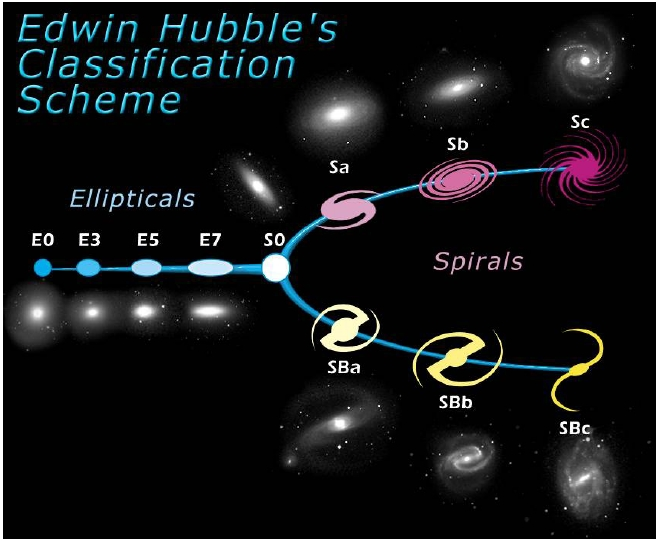
\includegraphics{figures/hubbleClass.jpg}}
\end{center}
\end{minipage}

\begin{minipage}[t]{16cm}
\begin{center}
\vskip -1in
     {\large \color{red}  Hubble's Morphological Classification}
\end{center}

\begin{itemize}
\item
Broadly, galaxies can be divided into ellipticals, spirals, and irregulars
\item
Broadly, spirals are divided into {\color{blue} normal and barred} (similar 
frequencies): S and SB
\item
The subclassification (a, b, or c) refers both to the {\color{blue}  size of the nucleus and the 
tightness of the spiral arms}. For example, the nucleus of an Sc galaxy is smaller 
than in an Sa galaxy, and the arms of the Sc are wrapped more loosely.
\item
The number and how tightly the spiral arms are wound are well correlated with other, 
large scale properties of the galaxies, such as the luminosity of the bulge relative 
to the disk and the amount of gas in the galaxy. This suggests that there 
are {\color{blue} global physical processes involved in spiral arms}.
\end{itemize}     

\end{minipage}}

\vfill 
\end{slide}
%------------------------------------------------------------------------------

\onepic{7}{-0.5}{-1.0}{0.8}{figures/variousClass.jpg}{}
%\onepic{7}{-0.5}{-1.2}{0.8}{ex1.jpg}{}
%\onepic{7}{-0.5}{-1.8}{0.8}{ex2.jpg}{}
\onepic{7}{-0.5}{-1.2}{0.7}{figures/ex3.jpg}{}
\onepic{7}{-0.5}{-1.2}{0.8}{figures/ex4.jpg}{}
\onepic{7}{-0.5}{-1.2}{0.7}{figures/ex5.jpg}{}

\onepic{7}{-0.5}{-1.8}{0.8}{figures/criteriaClass.jpg}{}
\onepic{7}{0.5}{-1.2}{0.7}{figures/other.jpg}{Galaxy types that didn't make it into
 the Hubble-Sandage system}






%------------------------------------------------------------------------------
% TWO-SIDED PAGE 
\begin{slide}

\hbox to \hsize{
\begin{minipage}[t]{7cm}
\begin{center}
\vskip -0.4in
\scalebox{0.55}{\hskip -1.8in 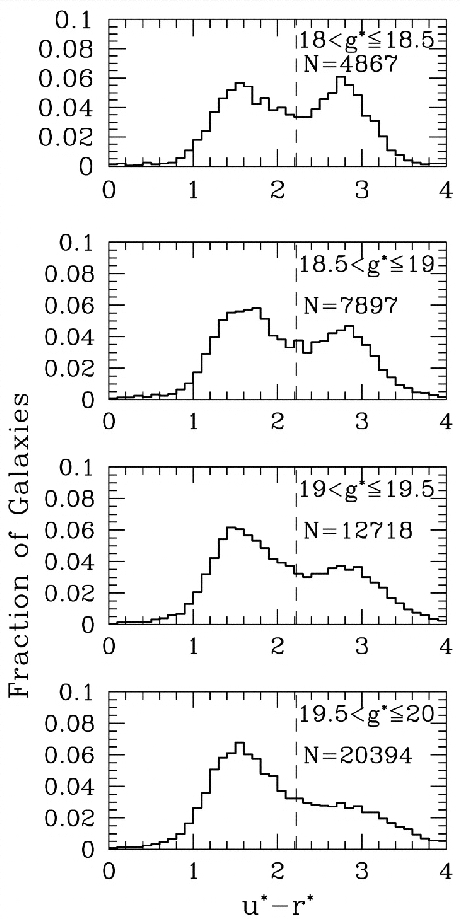
\includegraphics{figures/Strateva_ur.jpg}}


\end{center}
\end{minipage}

\begin{minipage}[t]{17cm}
\begin{center}
{\large \color{red} Colors are correlated with morphology }
\end{center}

\begin{itemize}
\item
Galaxies have bi-modal color distribution (e.g. SDSS $u-r$ color: the 
ratio of the UV and red fluxes): see histograms from Strateva et al. (2001, AJ, 122, 1861) 

\item
Colors correlated with shapes and profiles: blue galaxies tend to be 
spiral and red galaxies tend to be elliptical (there are deviants such
as e.g. ``anemic spirals'')
\item A good parametrization for shapes (i.e. intensity vs. radius $R$) 
is {\bf the Sersic index $n$:} \\
      $I(R) \propto \exp(-(R/R_e)^{1/n})$
\item 
{\color{blue} $n=1$: exponential profile}
\item
{\color{red} $n=4$: de Vaucouleurs profile}
\end{itemize}  

\end{minipage}}
\vfill 
\end{slide}
%------------------------------------------------------------------------------


\onepic{7}{0.5}{-0.8}{0.9}{figures/profiles.jpg}{Note the bulge contribution!}



%------------------------------------------------------------------------------

\begin{slide}
\begin{center}
{\large \color{red} 
       The light intensity distribution as a function of (elliptical) radius  }
\end{center}


Astronomers usually express brightness on a logarithmic (magnitude) scale
(well, at least optical astronomers do):
\eq{
         \log{I(R)}  = a - b\,R^{1/n}
}
Given an image of a galaxy (i.e. $I$ as a function of $R$), one can 
determine $a$, $b$ and $n$. Sometimes, $n$ is fixed as a function
of galaxy's morphology, and only $a$ and $b$ are fit to the data.

Sometimes, de Vaucouleurs profile is expressed as
\eq{
      I(R)= I_o \, 10^{-3.33\,[({R \over R_{1/2}})^{1/4} - 1]}
}
or for surface brightness (e.g. mag/arcsec$^2$)
\eq{
  \mu = -2.5\,\log{[I(R)]} = \mu_o + 8.33 \,[({R \over R_{1/2}})^{1/4} - 1]
}


\vfill
\end{slide}



%------------------------------------------------------------------------------

\begin{slide}
\begin{center}
{\large \color{red} 
       The light intensity distribution as a function of (elliptical) radius  }
\end{center}


Integral of $I(R)$ over the entire galaxy gives flux
\eq{
      F = 2 \pi \, \int_0^\infty I(R) \, R dR
}

This assumes that the profile was averaged in elliptical annuli. 
In general,
\eq{
      F = \int_0^\infty \int_0^{2\pi} I(R,\phi) \, R dR d\phi
}

Here, $I(R)$, and this $F$ is measured at some wavelength (and in 
some band). Integration over all wavelengths gives {\it bolometric}
flux. 

If flux $F$ is multiplied by $4 \pi D^2$, where $D$ is distance, 
one gets {\it luminosity}. Beware of units! 



\vfill
\end{slide}







%------------------------------------------------------------------------------

\begin{slide}
\begin{center}
{\large \color{red} 
       The light intensity distribution as a function of (elliptical) radius  }
\end{center}

{\color{blue} \bf Freeman's law:} when $\mu(R)$ is extrapolated
to the center of the galaxy ($R$=0, and excluding the bulge contribution), 
one gets a similar answer (to within 40-50\%) for all spiral galaxies!


This all (i.e. exp. profile and Freeman's law) applies to disks
of spiral galaxies. What about (luminous) halo? 

The answer depends on tracer; for the Milky Way
\begin{itemize}
\item
  {\color{blue} globular clusters}: $I(R) \propto R^{-3.5}$
\item
  {\color{red} RR Lyrae}: $I(R) \propto R^{-3.0}$
\end{itemize}


\vfill
\end{slide}


%------------------------------------------------------------------------------
% TWO-SIDED PAGE 
\begin{slide}

\hbox to \hsize{
\begin{minipage}[t]{13cm}
\begin{center}
\vskip 0.1in
\scalebox{0.45}{\hskip -1.8in 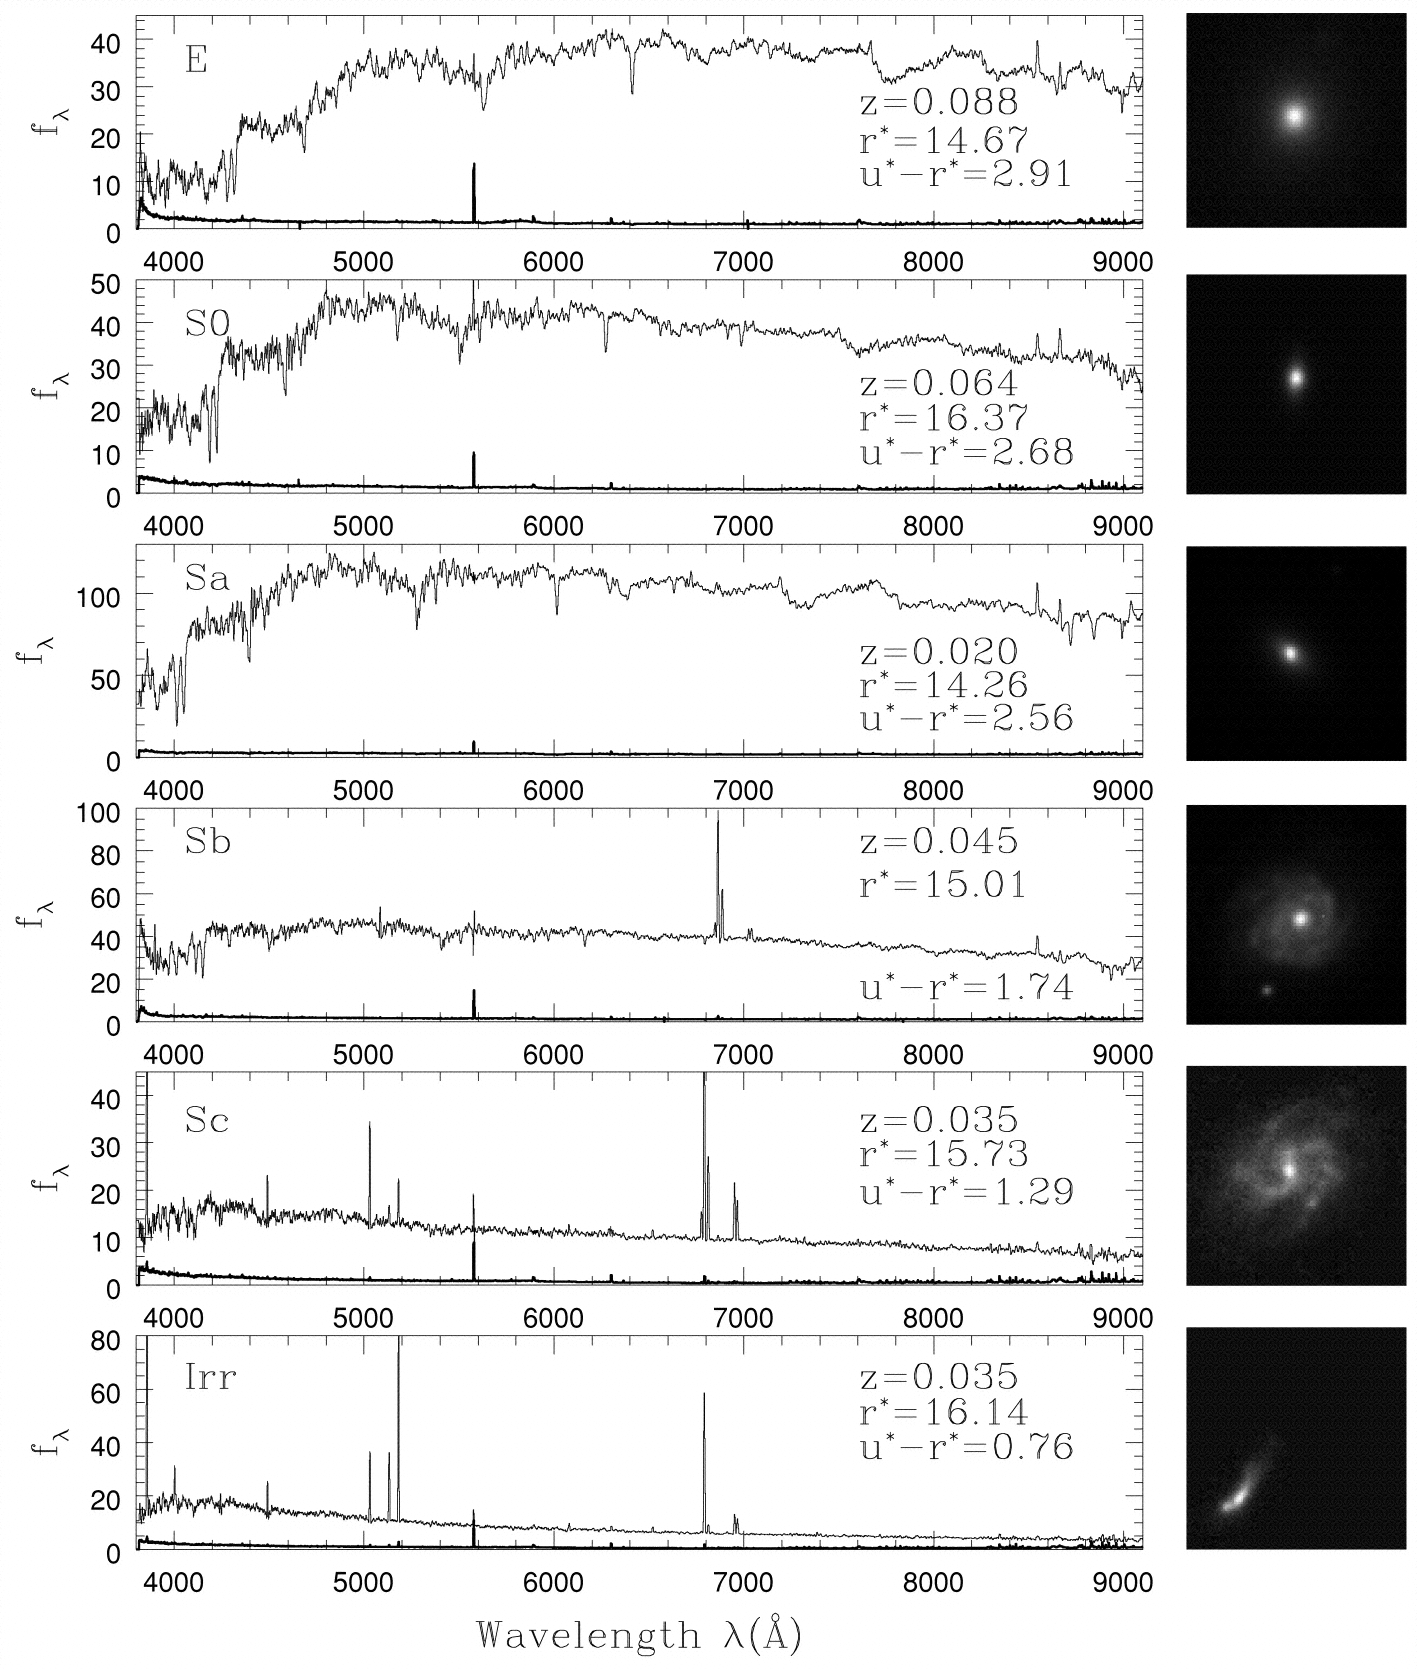
\includegraphics{figures/Strateva_fg4.jpg}}

\end{center}
\end{minipage}

\begin{minipage}[t]{11.5cm}

\begin{itemize}
\item
{\large \color{blue} Spectra are correlated with morphology}
\item
Galaxies with weak blue flux tend to be ellipticals (consistent with 
conclusions based on colors, of course)
\item
Galaxies with emission lines tend to be spiral galaxies (though
not all)
\item Both AGNs and star-forming galaxies show emission lines: 
  {\color{blue} How do we separate AGNs from star-forming galaxies?}
  Using the emission line ratios (which are also correlated with
  colors and shapes) (next time...)
\end{itemize}  

\end{minipage}}
\vfill 
\end{slide}
%------------------------------------------------------------------------------


%------------------------------------------------------------------------------

\begin{slide}
\begin{center}
{\large \color{red} 
             Rotation of Stars in the Disks of Spiral Galaxies }
\end{center}

\begin{itemize}
\item Most stars in spiral galaxies are concentrated in fairly thin disks
\item Stars move around the galaxy center -- described by the rotation (circular
     velocity) curve $v_c(R)$
\item The shape of rotation curve depends on the distribution of enclosed
      mass -- e.g. for a point mass $v_c(R) \propto 1/\sqrt{R}$
\item In general, $v^2_c(R) = R \, (d\Phi(R)/dR)$, where $\Phi$ is the gravitational
      potential ($\Phi$ follows from the mass density profile via Poisson 
      equation)
\item We know the disk light intensity profile; we can assume that mass is 
      following light and predict $v_c(R)$ for an exponential disk; but...
\end{itemize}     
 
\vfill
\end{slide}


\onepic{7}{-0.5}{-1.2}{0.95}{figures/rotcurve.jpg}{}


%------------------------------------------------------------------------------

\begin{slide}
\begin{center}
{\large \color{red} 
             Rotation of Stars in the Disks of Spiral Galaxies }
\end{center}


The prediction for rotation curve in an infinitely thin 
exponential disk (the previous slide) involves (somewhat)
complicated Bessel functions. A much simpler, but still
decent approximation is 
\eq{
      v_c(R) = 0.876 \sqrt{GM \over R_e} \sqrt{ r^{1.3} \over 1 + r^{2.3}}
}
where $R_e$ is the scale length ($I(R) \propto$ exp($-R/R_e$)), and
$r = 0.533 R/R_e$. 

Note that for $R >> R_e$, $v_c(R) \propto 1/\sqrt{R}$

FYI: if $M$ is measured in solar masses ($M_\odot$), $R$ in pc, 
$v_c$ in km/s, then the gravitational constant is $G=233$

{\color{blue} What do we get from observations?}

\vfill
\end{slide}




%------------------------------------------------------------------------------

\begin{slide}
\begin{center}
{\large \color{red} 
           Measurements of the Rotation Curve}
\end{center}


The circular speed can be determined as a function of radius
by measuring the redshift of emission lines of the gas contained
in the disk:

{\color{blue} Hot stars ionize gas:} hydrogen emission lines (e.g. $H_\alpha$) in
the optical

{\color{blue} Neutral atomic hydrogen gas}: hyperfine structure transition
(due to flip in electron spin) leads to 21 cm radio line




\vfill
\end{slide}


\onepic{7}{0.5}{-1.2}{0.9}{figures/rubin.jpg}{$H_\alpha$ measurements}




%------------------------------------------------------------------------------
% TWO-SIDED PAGE 
\begin{slide}

\hbox to \hsize{
\begin{minipage}[t]{8cm}
\begin{center}
\vskip 0.2in
\scalebox{0.8}{\hskip -1.4in 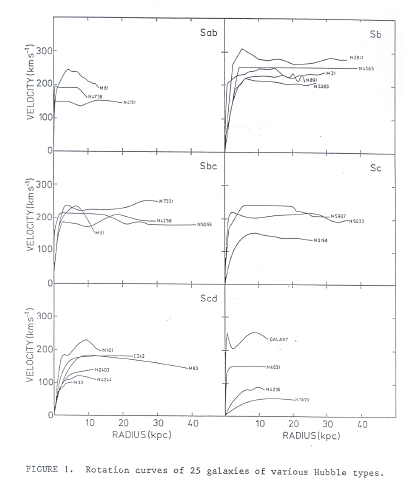
\includegraphics{figures/rotvel21cm.jpg}}
From A. Bosma's PhD Thesis (1978).
\end{center}
\end{minipage}

\begin{minipage}[t]{16cm}
\begin{center}
\vskip -1in
     {\large \color{red}  ``Flat'' rotation curves}
\end{center}

\begin{itemize}
\item
The measurements show that rotation curves are ``flat'' -- they are
not approching the $v_c(R) \propto 1/\sqrt{R}$ behavior expected in 
the outer parts of disks
\item
Therefore, {\color{blue} there must be an invisible galaxy component that 
is capable of producing gravitational force}
\item
Earlier (1930's) suggested by Fritz Zwicky, became an accepted view after
Rubin's work
\item
While, in principle, this discrepancy could also be due to a different
gravitational law (i.e. force that is not $\propto 1/R^2$), the modern
data, including cosmic microwave background measurements, suggest
that indeed that is a {\color{blue}  ``dark matter''} component contributing
{\color{red} $\sim$5 more gravitational force than stars and gas combined!}

\end{itemize}     

\end{minipage}}

\vfill 
\end{slide}
%------------------------------------------------------------------------------




\onepic{7}{0.0}{-1.8}{0.9}{figures/DMhalo.jpg}{}
\onepic{7}{0.0}{-0.8}{0.98}{figures/DMhalo2.jpg}{}





%------------------------------------------------------------------------------

\begin{slide}
\begin{center}
{\large \color{red} 
           The Tully-Fisher Relation (more in Lecture 5)}
\end{center}

The (maximum, the flat part value) rotation velocity is related to  
galaxy's luminosity: 
\eq{
              M_B = A \, \log{v_c} + B 
}
where $A\sim-10$ and $B\sim3$ depend slightly on galaxy's
morphological type.

Another way of expressing the same correlation
\eq{
                 L \propto v_c^{-0.4A} \propto v_c^4 
}

{\color{red} Why?} From the virial theorem, $v^2 \propto M/R$.
Also, $L \propto I R^2$, and hence
\eq{
      L \propto ({M \over L})^{-2} I^{-1} v^4
}
Since $I\sim$const. (Freeman's law), the Tully-Fisher relation implies
that $({M \over L}) \sim$ const. for spiral galaxies ($\sim$30 in the B 
band, and in solar units) 

\vfill
\end{slide}





%------------------------------------------------------------------------------
\begin{slide}
\begin{center}
\vskip -0.1in
\scalebox{0.5}{\hskip 0.0in 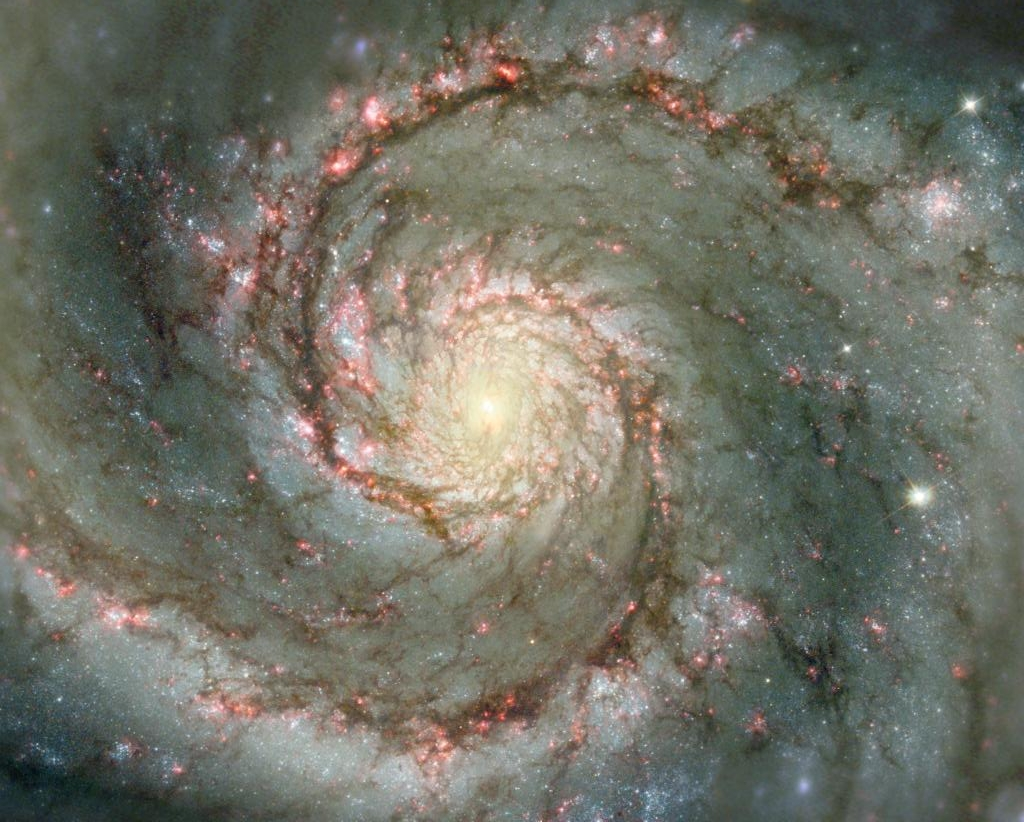
\includegraphics{figures/M51_HST.jpg}}
\end{center}

\begin{center}
\vskip -0.3in
Lord Rosse in 1845 ``discovered'' spiral structure in M51 (this is an HST image of M51)

\end{center}

\vfill
\end{slide}

%------------------------------------------------------------------------------


%------------------------------------------------------------------------------
\begin{slide}
\begin{center}
\vskip -0.1in
\scalebox{1.15}{\hskip 0.0in 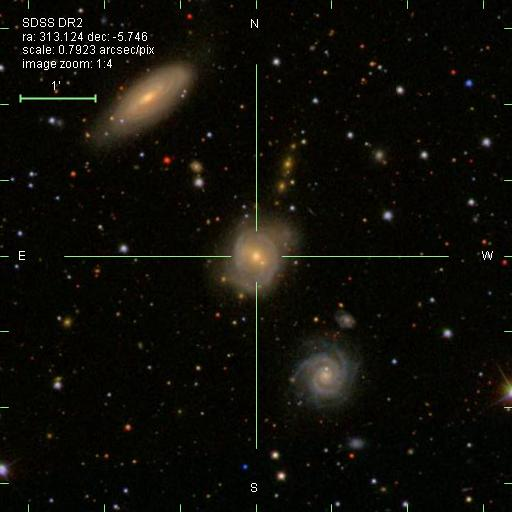
\includegraphics{figures/diskIns2.jpg}}
\end{center}

\begin{center}
\vskip -0.3in
{\large Not all spirals are alike!}	
\end{center}

\vfill
\end{slide}

%------------------------------------------------------------------------------


%------------------------------------------------------------------------------
\begin{slide}
\begin{center}
\vskip -0.1in
\scalebox{0.9}{\hskip 0.0in 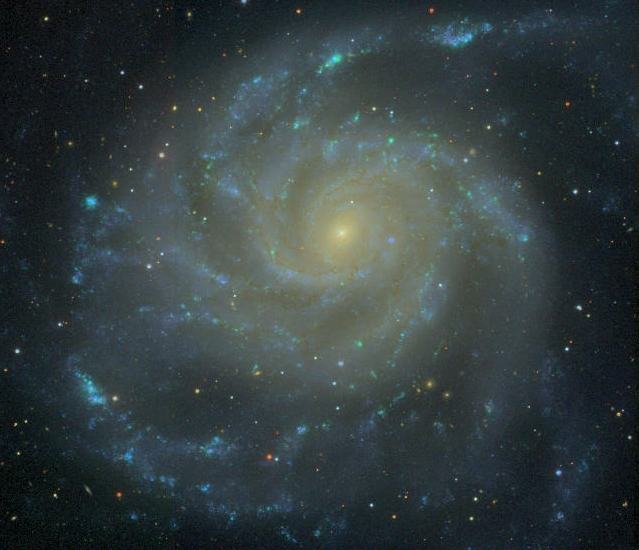
\includegraphics{figures/diskIns6.jpg}}
\end{center}


\vfill
\end{slide}

%------------------------------------------------------------------------------



%------------------------------------------------------------------------------
\begin{slide}
\begin{center}
\vskip -0.9in
\scalebox{0.75}{\hskip 0.0in 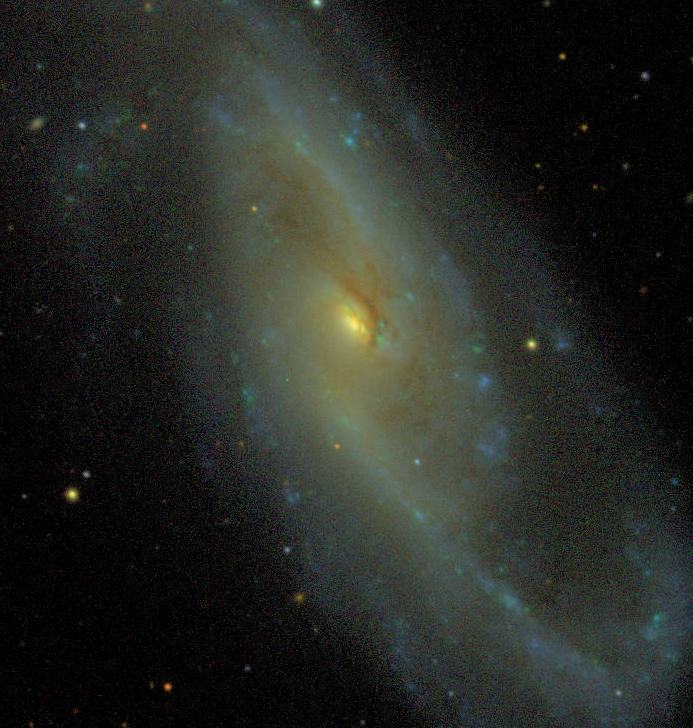
\includegraphics{figures/diskIns5.jpg}}
\end{center}


\vfill
\end{slide}

%------------------------------------------------------------------------------





%------------------------------------------------------------------------------
\begin{slide}
\begin{center}
\vskip -0.1in
\scalebox{0.9}{\hskip 0.0in 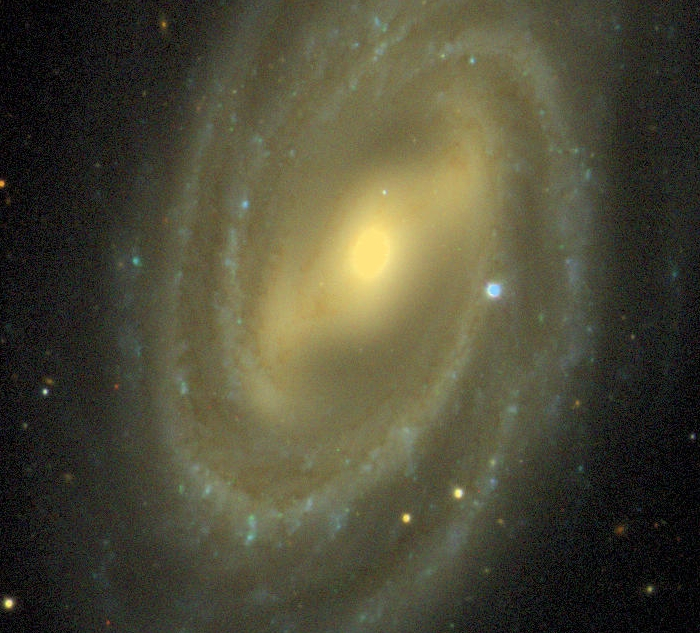
\includegraphics{figures/diskIns3.jpg}}
\end{center}


\vfill
\end{slide}

%------------------------------------------------------------------------------







%------------------------------------------------------------------------------
% TWO-SIDED PAGE 
\begin{slide}

\hbox to \hsize{
\begin{minipage}[t]{8cm}
\begin{center}
\vskip 0.7in
\scalebox{0.95}{\hskip -0.8in 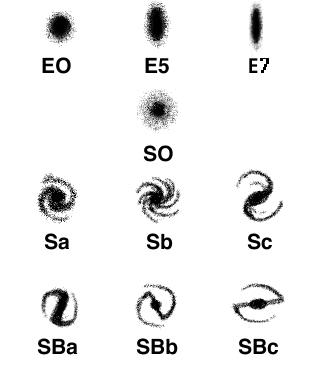
\includegraphics{figures/hubclass.jpg}}
\end{center}
\end{minipage}

\begin{minipage}[t]{16cm}
\begin{center}
\vskip -1in
     {\large \color{red}  Hubble's Morphological Classification}
\end{center}

\begin{itemize}
\item
Broadly, galaxies can be divided into ellipticals, spirals, and irregulars
\item
Broadly, spirals are divided into {\color{blue} normal and barred} (similar 
frequencies): S and SB
\item
The subclassification (a, b, or c) refers both to the {\color{blue}  size of the nucleus and the 
tightness of the spiral arms}. For example, the nucleus of an Sc galaxy is smaller 
than in an Sa galaxy, and the arms of the Sc are wrapped more loosely.
\item
The number and how tightly the spiral arms are wound are well correlated with other, 
large scale properties of the galaxies, such as the luminosity of the bulge relative 
to the disk and the amount of gas in the galaxy. This suggests that there 
are {\color{blue} global physical processes involved in spiral arms}.
\end{itemize}     

\end{minipage}}

\vfill 
\end{slide}
%------------------------------------------------------------------------------



%------------------------------------------------------------------------------
\begin{slide}
\begin{center}
\vskip -0.1in
\scalebox{0.8}{\hskip -1.0in 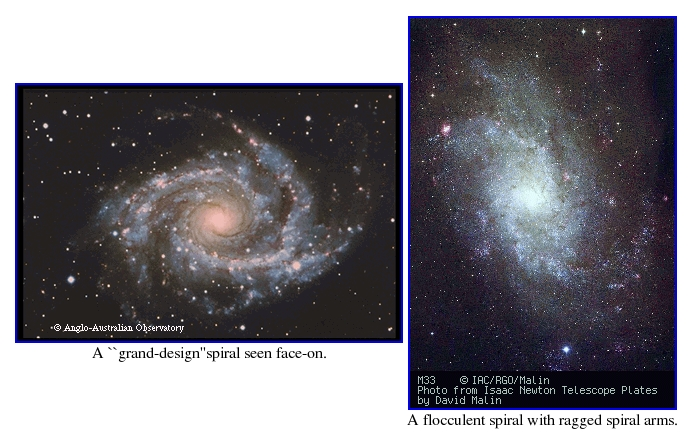
\includegraphics{figures/Wproblem4.jpg}}
\end{center}

\begin{center}
\vskip -0.3in

In addition to Hubble's classification, there are different types of 
spiral structure: {\color{blue} grand design} spirals, with clearly outlined 
and well organised {\color{red} globally correlated} spiral structure, and 
{\color{blue} flocculent} (fluffy) spirals with many small short {\color{red} 
globally uncorrelated} spiral arms

\end{center}

\vfill
\end{slide}

%------------------------------------------------------------------------------




%------------------------------------------------------------------------------
\begin{slide}
\begin{center}
\vskip 0.1in
\scalebox{1.1}{\hskip 0.0in 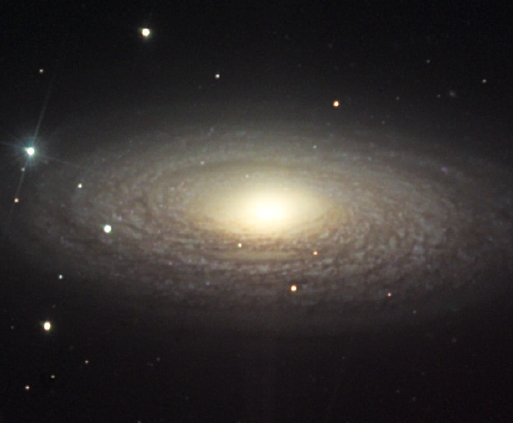
\includegraphics{figures/n2841.jpg}}
\end{center}



\vfill
\end{slide}

%------------------------------------------------------------------------------


%------------------------------------------------------------------------------
\begin{slide}

\begin{center}
{\large \color{red} Theories of Spiral Structure   }
\end{center}


Despite 50 years of work, spirals are not very well understood.
It seems clear now that {\color{blue} the spiral structure of galaxies 
is a complex problem} without any unique and tidy answer.

Differential rotation clearly plays a central role,
as well as global instabilities, stochastic spirals, and the shocks patterns that can 
arise in shearing gas disks when forced by bars.	

There are (at least) two popular theories, one of which is more commonly used to explain 
grand design spirals, the other for flocculent spirals.

But before proceeding: {\bf winding problem} (Lindblad)



\vfill
\end{slide}


%------------------------------------------------------------------------------
\begin{slide}
\begin{center}
{\large \color{red} Winding problem }
\end{center}

\begin{center}

\scalebox{0.95}{\hskip -0.0in 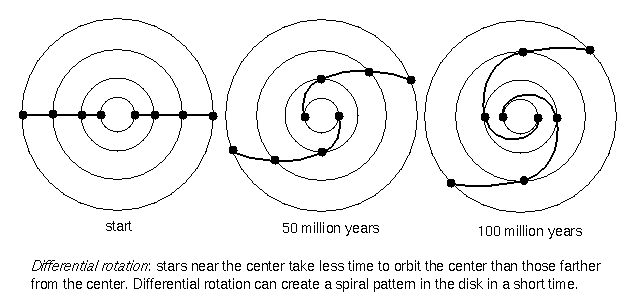
\includegraphics{figures/Wproblem1.jpg}}



\end{center}

\vfill
\end{slide}

%------------------------------------------------------------------------------

%------------------------------------------------------------------------------
\begin{slide}
\begin{center}
{\large \color{red} Winding problem }
\end{center}

\begin{center}

\scalebox{0.95}{\hskip -0.0in 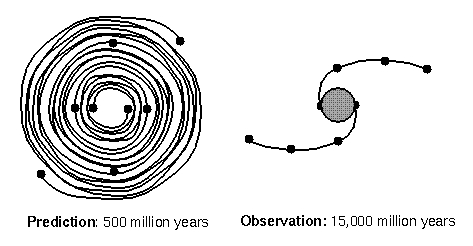
\includegraphics{figures/Wproblem2.jpg}}

{\color{blue} The problem: most spiral galaxies would be tightly
wound by now}, which is inconsistent with observations. 

{\color{blue} Spiral
arms cannot be a static structure} (i.e. at different times, arms
must be made of different stars)

\end{center}

\vfill
\end{slide}

%------------------------------------------------------------------------------


%------------------------------------------------------------------------------
% TWO-SIDED PAGE 
\begin{slide}

\hbox to \hsize{
\begin{minipage}[t]{11cm}
\begin{center}
\vskip 0.7in
\scalebox{0.90}{\hskip -1.1in 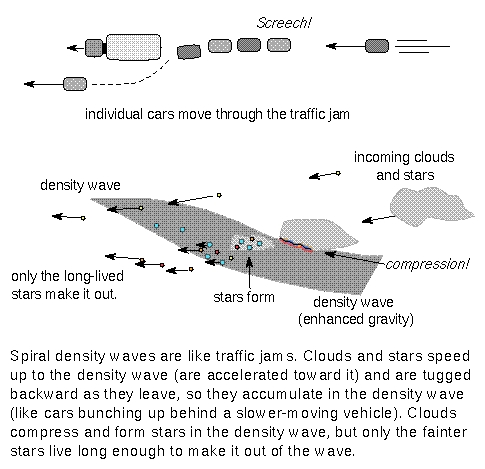
\includegraphics{figures/Wproblem3.jpg}}
\end{center}
\end{minipage}

\begin{minipage}[t]{11cm}
\begin{center}
\vskip -1in
     {\large \color{red}  Density Wave theory }
\end{center}

{\color{blue} C.C. Lin \& F. Shu (1964-66)}
\begin{itemize}
\item
This is the preferred model for grand design spirals. 
\item
The spiral arms are 
overdense regions which move around at a different 
speed than star: stars thus move in and out of the spiral arm 
\item
How these density waves are set up is unclear, but it may have to do with 
interactions. Once they are set up, they must last for a long enough time 
to be consistent with the observed number of spiral galaxies
\end{itemize}

\end{minipage}}

\vfill 
\end{slide}
%------------------------------------------------------------------------------


%------------------------------------------------------------------------------
\begin{slide}
\begin{center}
   {\large \color{red} Stochastic Self-Propagative Star Formation}
\end{center}

\begin{center}

\begin{itemize}
\vskip -0.3in
\item 
This model probably cannot explain grand design sprials, but it may account
for flocculent spiral structure. 
\vskip -0.3in
\item
Ongoing star formation triggers star formation in areas adjacent to it. As
the galaxy rotates, differential rotation leads to the appearance of a spiral pattern.
\end{itemize}


{\color{blue} {\it Spiral arms are made of short-lived massive blue stars!}}

\end{center}

\vfill
\end{slide}

%------------------------------------------------------------------------------





%------------------------------------------------------------------------------
\begin{slide}

\begin{center}
\vskip 1.2in
\scalebox{1.35}{\hskip -0.0in 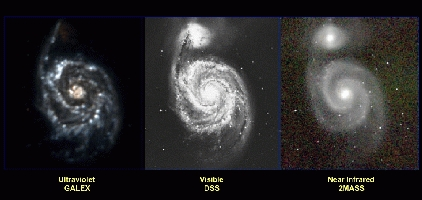
\includegraphics{figures/GALEX-M51.jpg}}

\end{center}

Note that the smaller galaxy (NGC 5195) is not visible in GALEX
image (left). 

{\bf \color{blue}  The spiral structure is associated with (short-lived) hot stars.}
 
\vfill
\end{slide}

%------------------------------------------------------------------------------


% Add stoch.jpg


\onepic{7}{0.5}{-1.2}{0.9}{figures/stoch.jpg}{}




%------------------------------------------------------------------------------
\begin{slide}

\begin{center}
\scalebox{0.55}{\hskip -0.8in 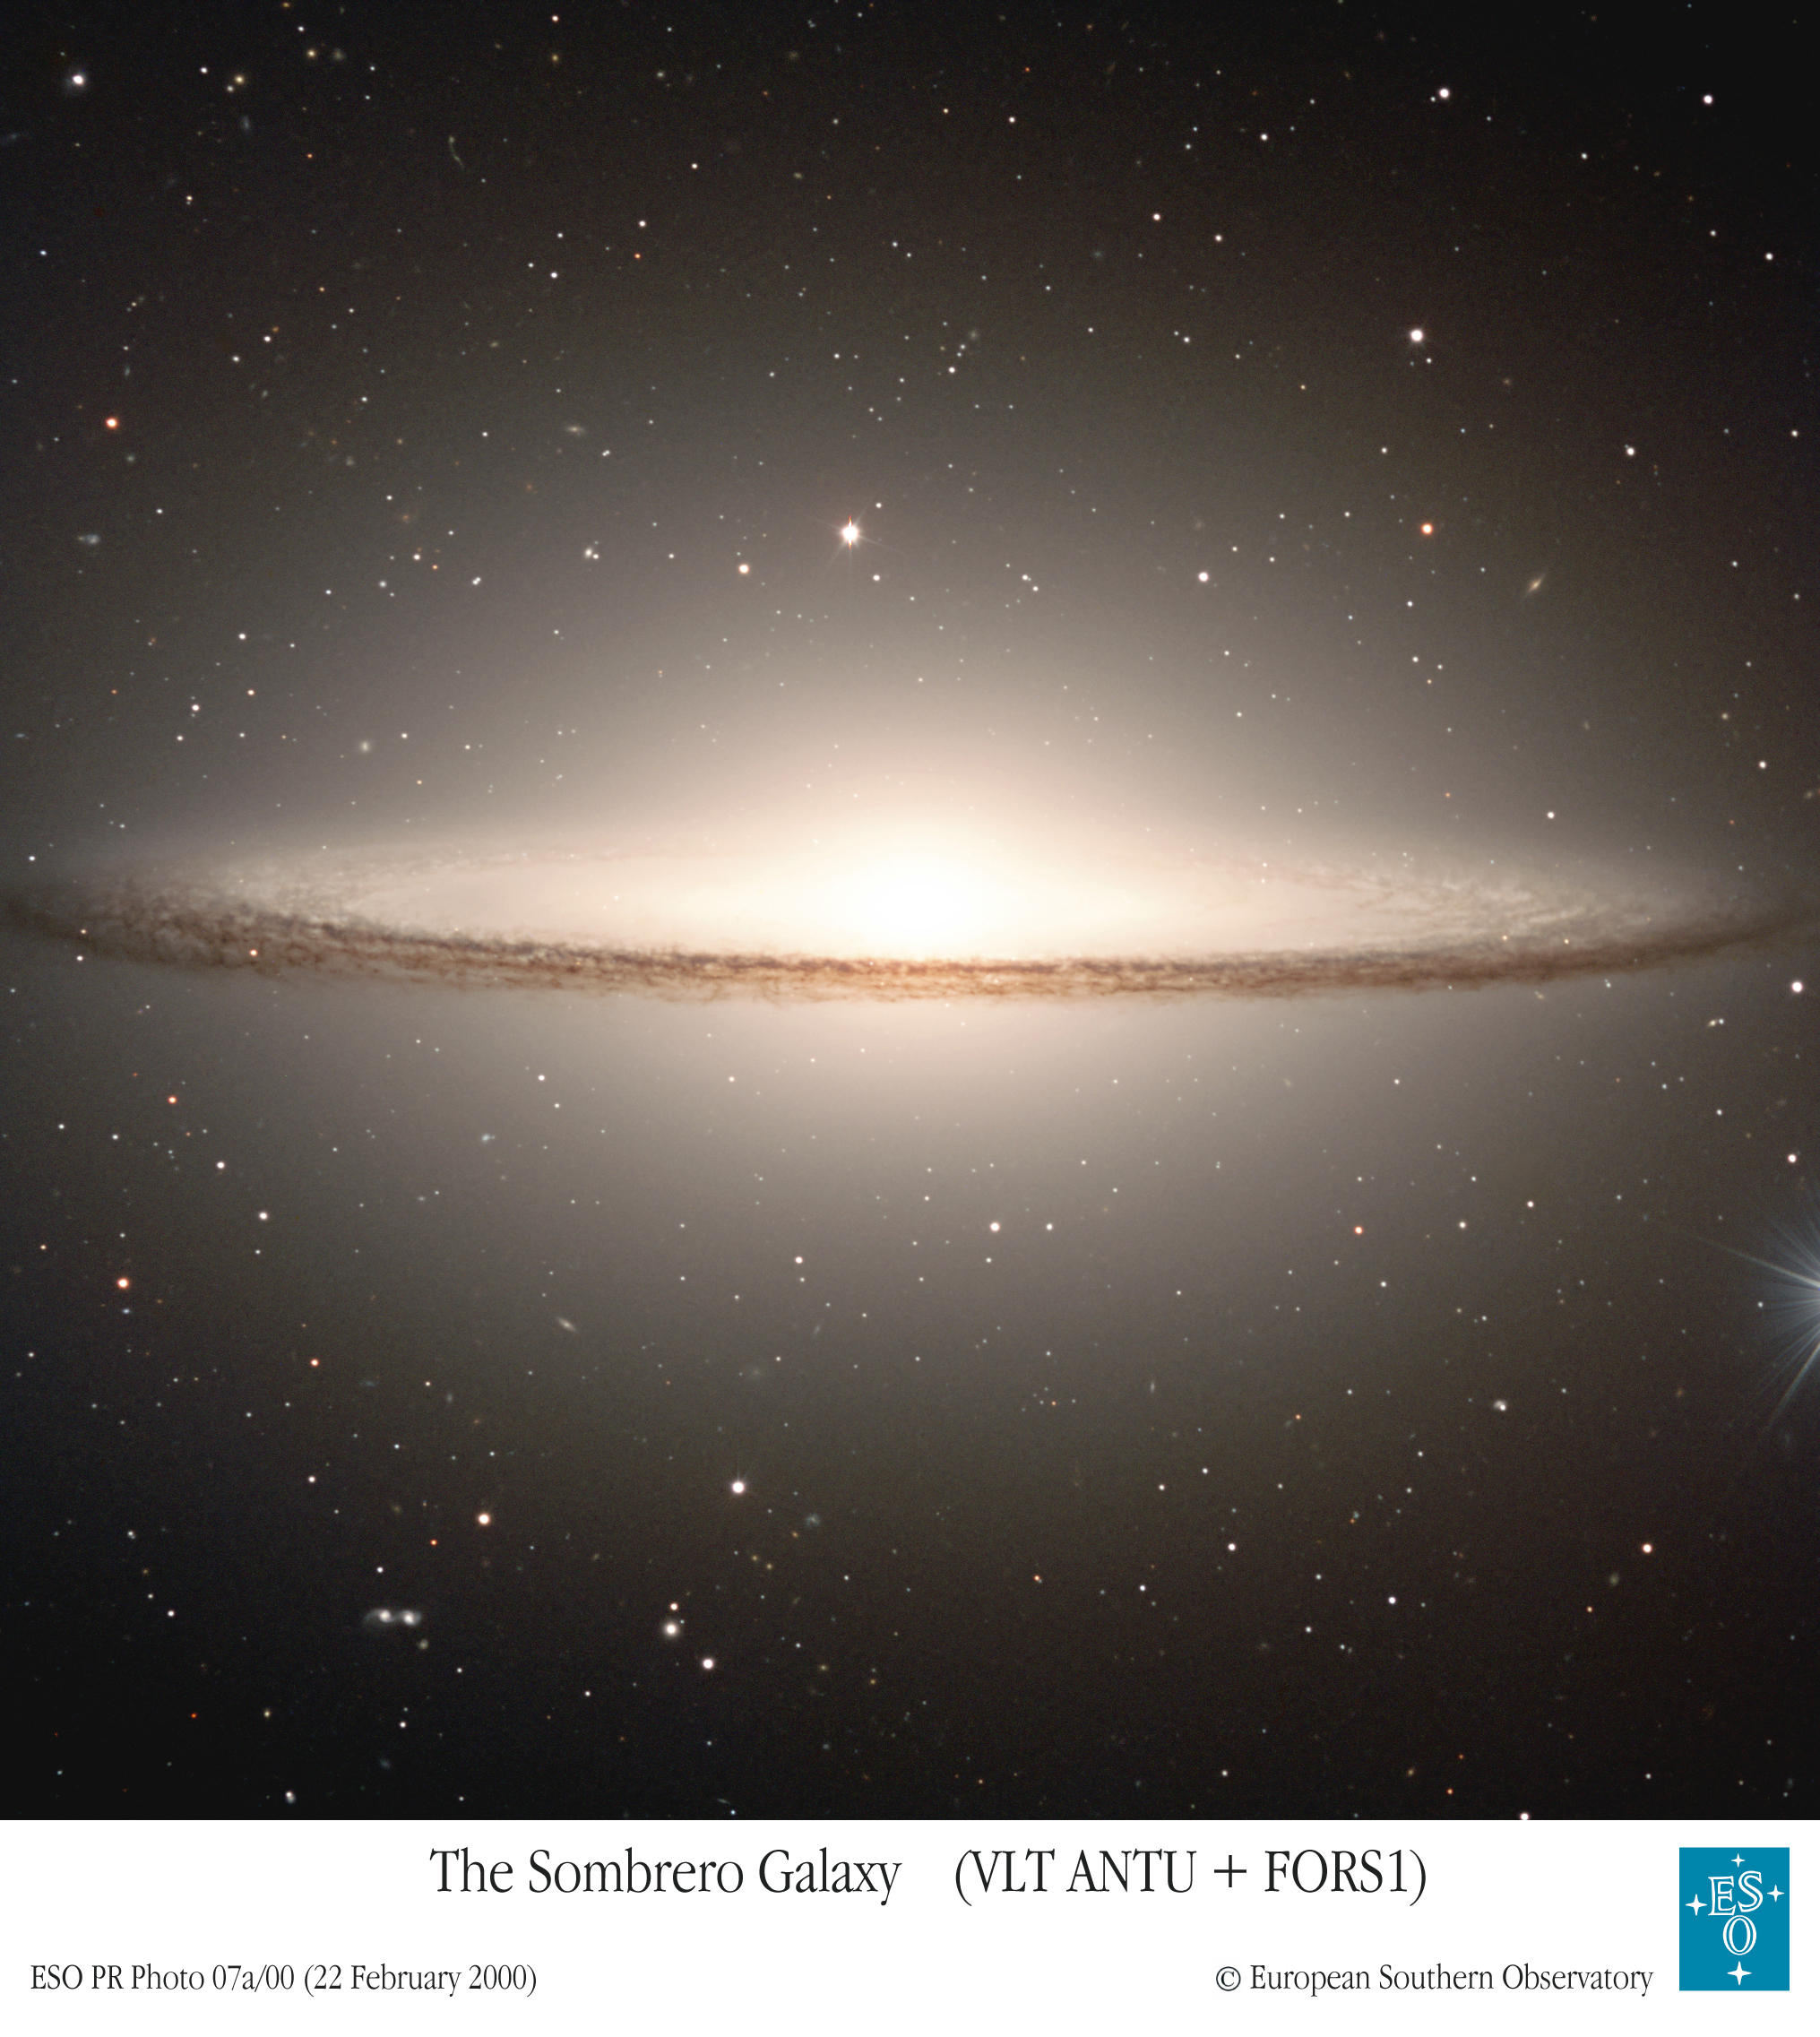
\includegraphics{figures/sombrero.jpg}}
\end{center}

{\bf \color{blue}  Disks contain a lot of dust!} Spiral arms are almost exclusively
seen in disks with a lot of gas and dust, unlike bars which are often seen
in galaxies without ISM. {\color{blue} Bars are not a wave of star formation -- they are
orbital features.}
 
\vfill
\end{slide}

%------------------------------------------------------------------------------



%------------------------------------------------------------------------------
\begin{slide}
\begin{center}
{\color{red} To remember:}
\end{center}

\begin{itemize}
\item
Spiral arms are not static structure (winding problem)
\item
Not all spirals are alike: more than one pattern
\item
Not clear if transient or quasy-steady phenomenon; 
the extent controlled by Lindblad resonances 
\item 
The appearance dominated by young luminous blue stars, but
the overall density of {\it all} stars is elevated by
10-20\% in spiral arms 
\end{itemize}

\vfill
\end{slide}

%------------------------------------------------------------------------------


%------------------------------------------------------------------------------
\begin{slide}
\begin{center}
{\color{red} Types of Elliptical Galaxies}
\end{center}


{\color{blue} You've seen one, you've seen them all!} {\color{red} Not true.}


\begin{itemize}
\item {\color{blue}Giant luminous ellipticals, cD:} the largest (1 Mpc!) and most luminous galaxies,
      very large mass-to-light ratios (lots of dark matter), masses $10^{13}-10^{14}$ M$_\odot$
\item {\color{blue}Normal ellipticals:} most numerous, masses $10^{8}-10^{13}$ M$_\odot$
\item {\color{blue}Dwarf ellipticals:} masses $10^{7}-10^{9}$ M$_\odot$ -- fundamentally different from all 
 other ellipticals by having low surface brightness and lower metallicity
\item {\color{blue}Dwarf spheroidals:} masses $10^{7}-10^{8}$ M$_\odot$, the low-mass end of normal ellipticals
\item {\color{blue}Blue compact dwarf galaxies:} masses $\sim10^{9}$ M$_\odot$, similar to dwarf ellipticals
     but unusually blue colors -- indicates ongoung star formation (yes, they do have lots of
     gas); very low mass-to-light ratios
\end{itemize}



\vfill
\end{slide}

%------------------------------------------------------------------------------


%------------------------------------------------------------------------------

\begin{slide}
\begin{center}
{\large \color{red} 
           The Faber-Jackson Relation (more in Lecture 5)}
\end{center}

Remember the Tully-Fisher Relation for spiral galaxies?
\eq{
                 L \propto v_c^4 
}
Here $v_c$ is the {\color{red} rotational} velocity. 

Do we have an analogous relation for elliptical galaxies? 

Unlike spiral galaxies, {\color{red} elliptical galaxies don't rotate} -- 
use the velocity dispersion, $\sigma$, instead.

The Faber-Jackson Relation:
\eq{
                 L \propto \sigma^4 
}
Actually, the exponent varies from 3 to 5, depending on sample
and band.

The scatter in the FJ relation is decreased by adding another physical parameter --
{\color{red} the fundamental plane}:
\eq{
                 L \propto \sigma^{2.65} r_e^{0.65} 
}



\vfill
\end{slide}



%------------------------------------------------------------------------------
\begin{slide}
\begin{center}
\vskip -0.1in
\scalebox{1.0}{\hskip 0.0in 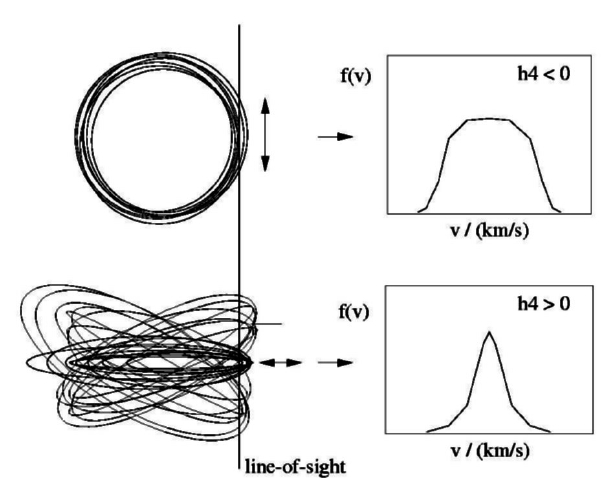
\includegraphics{figures/veldisp.jpg}}
\end{center}

\begin{center}
\vskip -0.3in
The {\color{blue} velocity dispersion} is the width of the velocity distribution.
\end{center}

\vfill
\end{slide}

%------------------------------------------------------------------------------


%------------------------------------------------------------------------------

\begin{slide}
\begin{center}
\vskip -0.1in
\scalebox{0.88}{\hskip -1in 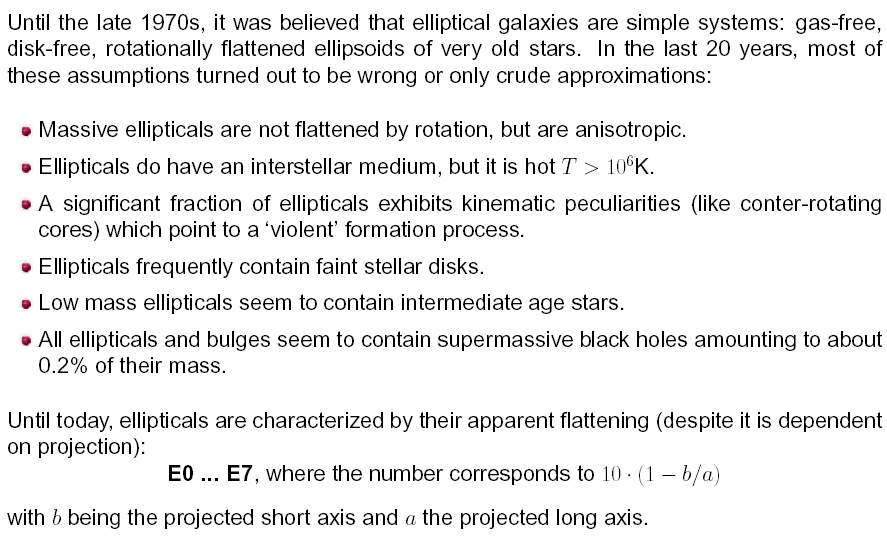
\includegraphics{figures/introE.jpg}}
\end{center}


\vfill
\end{slide}

%------------------------------------------------------------------------------

\begin{slide}
\begin{center}
{\large \color{red} 
           The Light Profiles of Elliptical Galaxies }
\end{center}




Remember the Sersic profile: $I(R) \propto \exp(-(R/R_e)^{1/n})$?
For elliptical galaxies $n=4$ -- de Vaucouleurs profile:
\eq{
      I(R)= I_o \, 10^{-3.33\,[({R \over R_{1/2}})^{1/4} - 1]}
}

Another commonly used profiles are King models (isothermal sphere)
and Jaffe's spheres. The latter has almost identical light profile
as de Vaucouleurs profile, but the density law and gravitational 
potential are analytic:
\eq{
       \rho_L(r) = {L \over 4\pi r_o^3} \, \left({r_o \over r}\right)^2 \, {1 \over (1 + r_o/ r)^2}  
}

\eq{
         \Phi(r) = {GL \over r_o} \, \left({M \over L}\right) \ln{\left(1 \over 1 + r_o/ r\right)}
}

\vfill
\end{slide}

%------------------------------------------------------------------------------

\begin{slide}
\begin{center}
\vskip -0.1in
\scalebox{0.88}{\hskip -1in 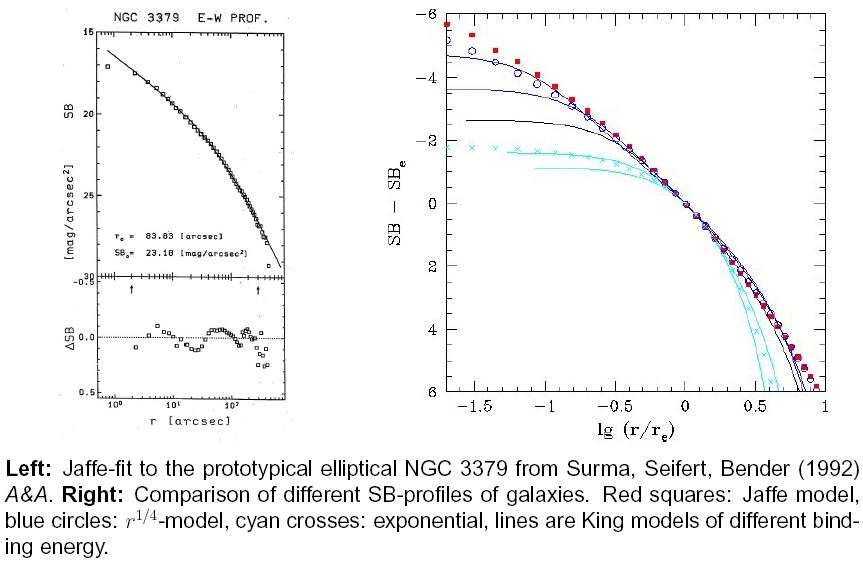
\includegraphics{figures/Eprofiles.jpg}}
\end{center}


\vfill
\end{slide}





%------------------------------------------------------------------------------
% TWO-SIDED PAGE 
\begin{slide}

\hbox to \hsize{
\begin{minipage}[t]{8cm}
\begin{center}
\vskip 0.7in
\scalebox{0.95}{\hskip -0.8in 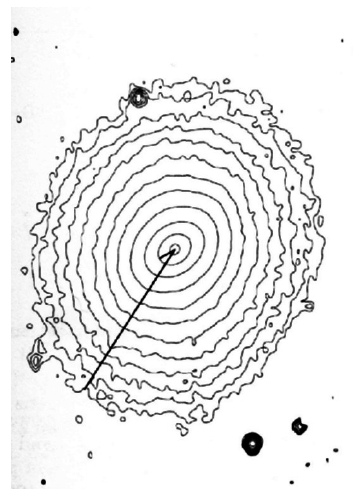
\includegraphics{figures/Eisotwist.jpg}}
\end{center}
\end{minipage}

\begin{minipage}[t]{16cm}
\begin{center}
\vskip -1in
     {\large \color{red}  True shapes of elliptical galaxies}
\end{center}

\begin{itemize}
\item
The classification of elliptical galaxies (E0--E7)is based on {\bf apparent} 
flattening: are the true shapes bi-axial (as expected for rotation), or 
triaxial (as expected for randomly distributed orbits)?
\item
{\color{blue} Elliptical galaxies are modestly triaxial} -- a:b:c $\sim$ 1:0.95:0.7 
(nearly {\it oblate},
a=b$>$c, like an UFO, as opposed to {\it prolate}, a$>$b=c, like a football)
\item 
We know that because of the effect called {\color{blue} ``isophote twist''}, which doesn't
happen for bi-axial shapes, only for triaxial
\item
Therefore, (most)  {\color{red} elliptical galaxies are {\bf NOT} supported by rotation}
\item
Isophotes are not exactly elliptical: {\it boxy} vs. {\it disky}. The latter can
be explained as a superposition of an elliptical bulge on a faint edge-on disk.
\end{itemize}     

\end{minipage}}

\vfill 
\end{slide}
%------------------------------------------------------------------------------



%------------------------------------------------------------------------------

\begin{slide}
\begin{center}
\vskip -0.1in
\scalebox{0.88}{\hskip -0.3in 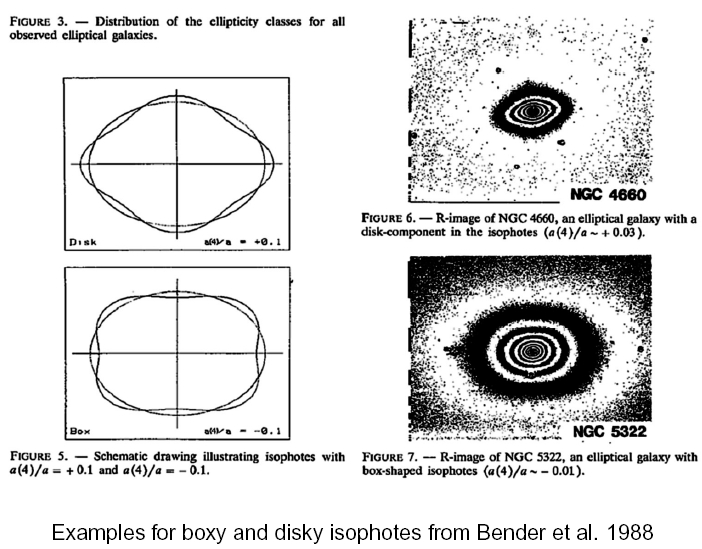
\includegraphics{figures/boxydisky.jpg}}
\end{center}


\vfill
\end{slide}




%------------------------------------------------------------------------------

\begin{slide}
The central regions of elliptical galaxies include two types of profiles:
{\bf cuspy cores} and {\bf power-law cores} 


\begin{center}
\vskip -0.1in
\scalebox{0.88}{\hskip -0.3in 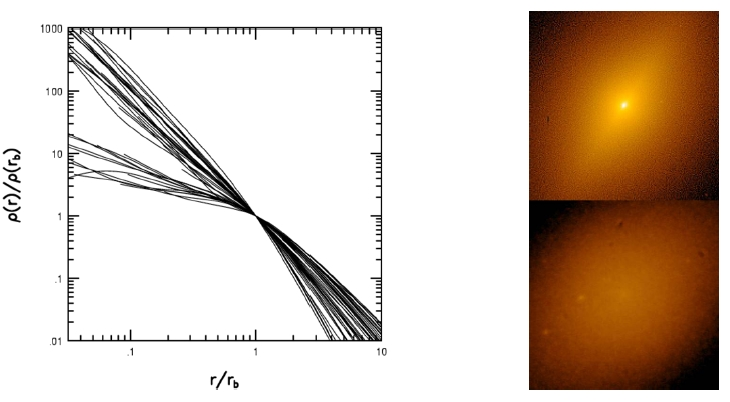
\includegraphics{figures/Ecores.jpg}}
\end{center}

\vfill
\end{slide}





%------------------------------------------------------------------------------

\begin{slide}
\begin{center}
{\large \color{red} 
                         Dark Matter in Elliptical Galaxies   (more in Lecture 10)   }
\end{center}

In the central part of elliptical galaxies there is no evidence for 
dark matter (mass-to-light ratio $\sim$5--10 in solar units -- typical
for old stellar populations). In the outer parts it is harder to 
find such evidence because there is no gas on circular orbit as is
the case for spiral galaxies.

Nevertheless, there are several methods that indicate {\color{blue}  the presence
of dark matter in elliptical galaxies:}
\begin{enumerate}
\item Analysis of stellar kinematics (detailed models of motion in 
    gravitational potential)
\item Gravitational lensing
\item X-ray halos (application of virial theorem)
\end{enumerate}


\vfill
\end{slide}



%------------------------------------------------------------------------------
% TWO-SIDED PAGE 
\begin{slide}

\hbox to \hsize{
\begin{minipage}[t]{12cm}
\begin{center}
\vskip -0.0in
\scalebox{0.8}{\hskip -0.0in 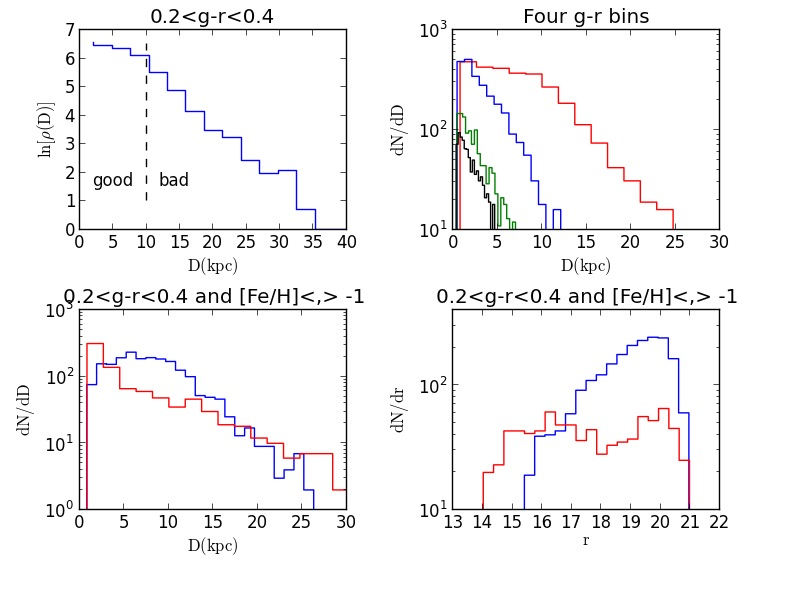
\includegraphics{figures/HW1_figure1.jpg}}
HW1 plot should look more or less like this one...
\end{center}

\end{minipage}

\begin{minipage}[t]{12cm}
\begin{center}
%{\large \color{red} ISM Medium }
\end{center}


\end{minipage}}
\vfill 
\end{slide}
%--------------------------------------------------------------------------------------------



\end{document}

